\documentclass[12pt]{article}

\usepackage{fontawesome}
\usepackage{hyperref}
\usepackage{xurl}
\usepackage{graphicx}
\usepackage{float}
\usepackage[tagged, highstructure]{accessibility}
\usepackage{bookmark}
\usepackage{enumitem}

\hypersetup{
    colorlinks=false,
    pdfborder={0 0 0},
    pdftitle={Web Security},
    pdfauthor={Adrianna Holden-Gouveia},
    pdfsubject={Information Security - Lab Assignment},
    pdflang={en-US},
    pdfkeywords={web security, Hacksplaining, tracking, browser fingerprinting, HTTPS, certificates}
}

% Configure PDF bookmarks for navigation
\bookmarksetup{
    numbered,
    open,
}

% Configure list spacing for better accessibility
\setlist{nosep}



\title{Web Security}
\author{
        Adrianna Holden-Gouveia \\
        Website: \href{https://aholdengouveia.name}{aholdengouveia.name}\\ 
        \date{\vspace{-5ex}}
        %Email: \href{mailto:admin@aholdengouveia.name}{admin@aholdengouveia.name} \\
%        \faLinkedin{: aholdengouveia} \\
        \faGithub {: aholdengouveia} \\
        \faTwitter {: aholdengouveia} \\
        }

%S\date{\today}


\begin{document}    

\maketitle

\section*{Accessibility Notice}
This document is also available in HTML format at:

Link: \href{https://aholdengouveia.name/InfoSec/labs/websecurity.html}{\textbf{\nolinkurl{https://aholdengouveia.name/InfoSec/labs/websecurity.html}}}

The HTML version provides enhanced accessibility features including keyboard navigation, screen reader support, responsive design, dark mode support, and high contrast options.


%\begin{abstract}
%This is a template for Linux Administration Lab work
%\end{abstract}
%\tableofcontents

\section*{Learning Outcomes}
By the end of this lab, you will be able to:
\begin{itemize}
    \item Explain how two common website attacks work, and how website owners can prevent them
    \item Test how easy your browser is to track, and compare ways to reduce tracking
    \item Explain what a website's certificate shows, and what browser certificate warnings mean
    \item Recommend ways people can protect themselves on the web
\end{itemize}

\section*{Lab Instructions}
Everything in this lab runs in your web browser, so you don't need to install anything. All the tools are linked under Resources.

You don't need to know how to code. Hacksplaining walks you through each step, and explains what's happening as you go.

\textbf{Only practice attacks on sites made for practice, like Hacksplaining.} Trying an attack on a real website without permission is illegal, even just to see if it works.

\subsection*{Screenshots}
This lab asks for 7 screenshots. Each screenshot should have your name, term, and year.  One of the easiest ways to do that is make a text document with your name and term/year on your computer and save it to use all term. Any screenshots that don't include this information won't be counted.

\begin{figure}[H]
    \centerline{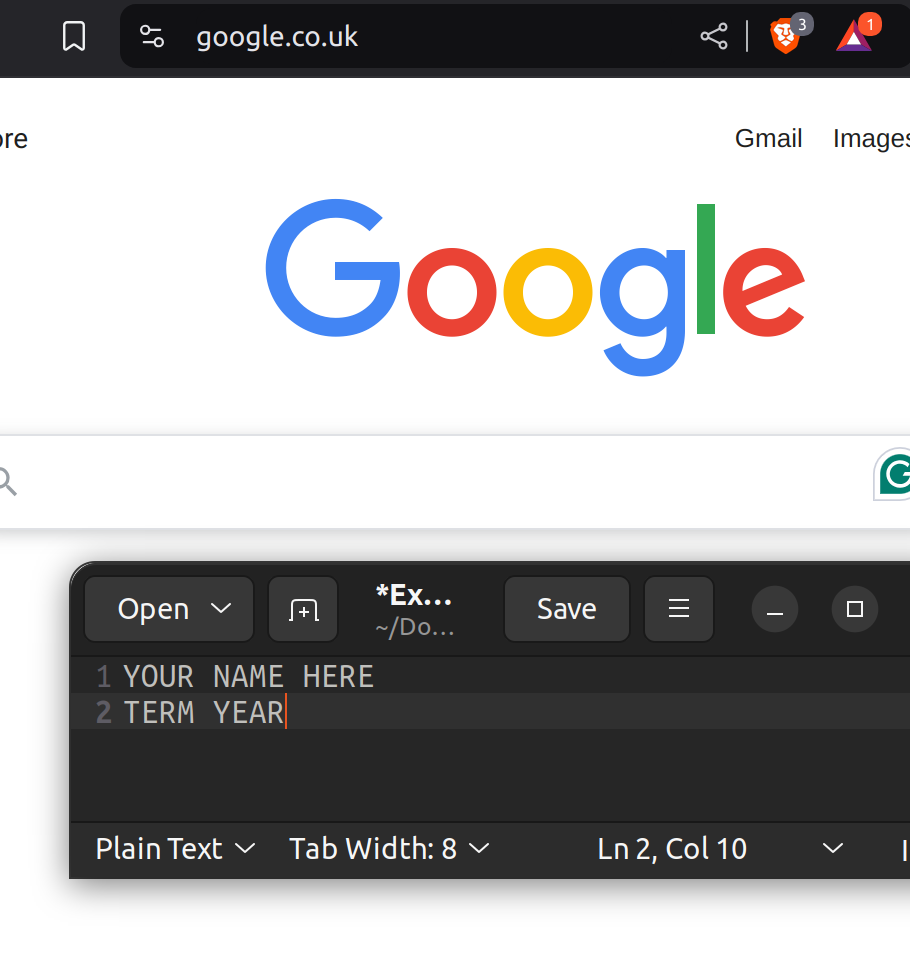
\includegraphics[scale=.2]{ExampleScreenshot.png}}
    \caption{This is an image of what each of your screenshots should look like}
    \alt{Example screenshot: a web browser showing the Google home page, with a small text editor window in front of it that says YOUR NAME HERE and TERM YEAR}
\end{figure}

\subsection*{Part 1: Attack a Practice Website}
Hacksplaining has short lessons where you attack a pretend website it runs, then learn how to fix it. Sign up for a free account. You can use your school email.

Pick \textbf{two} of these lessons:
\begin{itemize}
    \item SQL Injection
    \item Cross-site Scripting (reflected or stored)
    \item Password Mismanagement
    \item SSL Stripping
    \item Clickjacking
\end{itemize}
For each lesson:
\begin{enumerate}
    \item Finish the lesson and its quiz. Take a screenshot of the end of the lesson, showing it's complete.
    \item In your own words, explain how the attack works, as if you were telling a friend who doesn't work in IT.
    \item What could an attacker get or do with this attack? Who gets hurt: the website, its users, or both?
    \item How can the website's owner prevent it?
\end{enumerate}

\subsection*{Part 2: How Trackable Is Your Browser?}
EFF's Cover Your Tracks tests how websites and advertisers see your browser, and how unique it looks. No account is needed.
\begin{enumerate}[start=5]
    \item Run the test in the browser you use most. Take a screenshot of the results.
    \item Run it again with a different setup, such as a private window, a different browser, or your phone. Take a screenshot of the results.
    \item For each test, write down the browser and setup you used, whether it blocked tracking ads and invisible trackers, and whether your fingerprint was unique.
    \item What changed between the two tests? Which setup protected you better?
    \item Pick one thing the results showed about your browser, such as your screen size, time zone, or fonts. Why would a tracker want to know this?
\end{enumerate}

\subsection*{Part 3: Certificates and Browser Warnings}
Every HTTPS website has a certificate, which proves the website is who it says it is.
\begin{enumerate}[start=10]
    \item Pick 2 websites you use often. Select the padlock (or the icon next to the address), and find the certificate. Take a screenshot of each one.
    \item For each website, write down who issued the certificate, when it starts and expires, and how many days it lasts. A calendar or a date calculator website is fine for counting days.
    \item Were the two certificates from the same issuer? Did they last the same length of time? Why do you think certificates are getting shorter?
\end{enumerate}
badssl.com is a website made for testing. It has pages with broken certificates on purpose, so you can see the warnings safely. Visit each of these pages, and \textbf{don't} click through the warnings:
\begin{itemize}
    \item \nolinkurl{https://expired.badssl.com}
    \item \nolinkurl{https://self-signed.badssl.com}
    \item \nolinkurl{https://wrong.host.badssl.com}
    \item \nolinkurl{https://untrusted-root.badssl.com}
\end{itemize}
\begin{enumerate}[start=13]
    \item Take a screenshot of one of the warnings.
    \item For each page, explain in your own words what's wrong with the certificate, and why your browser warned you.
    \item If you saw a warning like this on your bank's website, what would you do? Why?
\end{enumerate}

\subsection*{Part 4: Your Advice}
\begin{enumerate}[start=16]
    \item Based on this lab, write 3 tips to help a friend or family member stay safer on the web. For each tip, explain which part of the lab it came from.
\end{enumerate}

\section*{Deliverables}
One file that includes:
\begin{itemize}
    \item Part 1: your 2 Hacksplaining screenshots, and your answers for each lesson
    \item Part 2: your 2 Cover Your Tracks screenshots, and your answers
    \item Part 3: your 2 certificate screenshots, your badssl.com warning screenshot, and your answers
    \item Part 4: your 3 tips
\end{itemize}

\section*{Resources}
References, a video, a PowerPoint and some notes are available at my website
Link: \href{https://www.aholdengouveia.name/InfoSec/WebSecurity.html}{\textbf{\nolinkurl{https://www.aholdengouveia.name/InfoSec/WebSecurity.html}}}

Hacksplaining lessons, for Part 1
Link: \href{https://www.hacksplaining.com/lessons}{\textbf{\nolinkurl{https://www.hacksplaining.com/lessons}}}

EFF's Cover Your Tracks, for Part 2
Link: \href{https://coveryourtracks.eff.org/}{\textbf{\nolinkurl{https://coveryourtracks.eff.org/}}}

badssl.com, for Part 3
Link: \href{https://badssl.com/}{\textbf{\nolinkurl{https://badssl.com/}}}

What HTTPS and certificates are
Link: \href{https://en.wikipedia.org/wiki/HTTPS}{\textbf{\nolinkurl{https://en.wikipedia.org/wiki/HTTPS}}}

The OWASP Top 10 web application security risks
Link: \href{https://owasp.org/www-project-top-ten/}{\textbf{\nolinkurl{https://owasp.org/www-project-top-ten/}}}

\end{document}
